\newpage
\section{Tinjauan Pustaka}

% berikut adalah fitur dari dataset buatkan tinjauan pusataka yang merepresentasikan fitur-fitur 
% Code Description
% - MEMBER_NO-b : ID Member
% - FFP_DATE : Frequent Flyer Program Join Date
% - FIRST_FLIGHT_DATE : Tanggal Penerbangan pertama
% - GENDER : Jenis Kelamin
% - FFP_TIER : Tier dari Frequent Flyer Program
% - WORK_CITY : Kota Asal
% - WORK_PROVINCE : Provinsi Asal
% - WORK_COUNTRY : Negara Asal
% - AGE : Umur Customer
% - LOAD_TIME : Tanggal data diambil
% - FLIGHT_COUNT : Jumlah penerbangan Customer
% - BP_SUM : Rencana Perjalanan
% - SUM_YR_1 : Fare Revenue
% - SUM_YR_2 : Votes Prices
% - SEG_KM_SUM : Total jarak(km) penerbangan yg sudah dilakukan
% - LAST_FLIGHT_DATE : Tanggal penerbangan terakhir
% - LAST_TO_END : Jarak waktu penerbangan terakhir ke pesanan penerbangan paling akhir
% - AVG_INTERVAL : Rata-rata jarak waktu
% - MAX_INTERVAL : Maksimal jarak waktu
% - EXCHANGE_COUNT : Jumlah penukaran
% - avg_discount : Rata rata discount yang didapat customer
% - Points_Sum : Jumlah poin yang didapat customer
% - Point_NotFlight : point yang tidak digunakan oleh members

\subsection{Frequent Flyer Program}
Frequent Flyer Program (FFP) adalah program loyalitas yang ditawarkan oleh maskapai penerbangan kepada pelanggan setia mereka. Program ini memberikan berbagai keuntungan, seperti akumulasi poin atau miles yang dapat ditukarkan dengan tiket penerbangan gratis, peningkatan kelas penerbangan, akses ke lounge bandara, dan layanan prioritas lainnya. FFP dirancang untuk mendorong pelanggan agar terus menggunakan layanan maskapai tertentu, sehingga meningkatkan retensi pelanggan dan loyalitas merek.

Program ini biasanya memiliki beberapa tingkatan atau tier, yang memberikan manfaat tambahan kepada anggota yang mencapai tingkat tertentu berdasarkan frekuensi penerbangan atau jumlah poin yang dikumpulkan. Dengan demikian, FFP tidak hanya memberikan insentif bagi pelanggan untuk terbang lebih sering, tetapi juga menciptakan hubungan jangka panjang antara maskapai dan pelanggannya.

\begin{figure}[H]
    \centering
    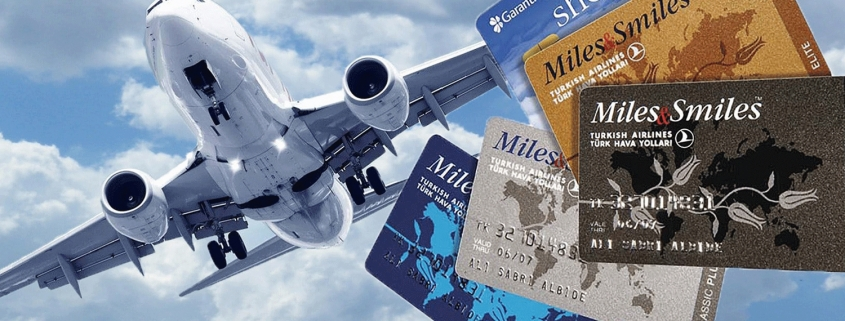
\includegraphics[width=0.6\textwidth]{gambar/ffp.jpg}
    \caption{Contoh Frequent Flyer Program}
    \label{fig:ffp}
\end{figure}

\subsection{EDA (Exploratory Data Analysis)}
Exploratory Data Analysis (EDA) adalah proses analisis data yang bertujuan untuk memahami struktur, pola, dan hubungan dalam dataset sebelum melakukan analisis lebih lanjut atau membangun model. EDA melibatkan penggunaan berbagai teknik statistik dan visualisasi untuk mengeksplorasi data, mengidentifikasi anomali, dan mendapatkan wawasan awal tentang karakteristik data.

Proses EDA biasanya mencakup langkah-langkah seperti:
\begin{itemize}
    \item \textbf{Pemeriksaan Data:} Memeriksa tipe data, nilai yang hilang, dan distribusi variabel.
    \item \textbf{Statistik Deskriptif:} Menghitung ukuran pusat (mean, median) dan ukuran dispersi (standar deviasi, rentang).
    \item \textbf{Visualisasi Data:} Menggunakan grafik seperti histogram, boxplot, dan scatter plot untuk memahami distribusi dan hubungan antar variabel.
    \item \textbf{Identifikasi Outlier:} Mendeteksi nilai-nilai yang tidak biasa yang dapat mempengaruhi analisis.
    \item \textbf{Korelasi:} Menganalisis hubungan antar variabel untuk mengidentifikasi pola yang mungkin ada.
\end{itemize}

EDA sangat penting dalam tahap awal analisis data karena membantu peneliti atau analis untuk memahami data secara mendalam, mengarahkan fokus pada area yang relevan, dan menginformasikan keputusan tentang teknik analisis yang akan digunakan selanjutnya. Dengan demikian, EDA merupakan langkah krusial dalam proses analisis data yang efektif.

\subsection{Data Preprocessing}
Data preprocessing adalah langkah penting dalam analisis data yang melibatkan pembersihan, transformasi, dan persiapan data sebelum digunakan dalam analisis atau pemodelan. Tujuan dari preprocessing adalah untuk memastikan bahwa data dalam kondisi yang baik, konsisten, dan siap untuk dianalisis. Langkah-langkah umum dalam data preprocessing meliputi:
\begin{itemize}
    \item \textbf{Pembersihan Data:} Menghapus atau memperbaiki data yang tidak lengkap, duplikat, atau tidak konsisten. Ini termasuk menangani nilai yang hilang, mengoreksi kesalahan pengetikan, dan menghapus outlier yang tidak relevan.
    \item \textbf{Transformasi Data:} Mengubah format data agar sesuai dengan kebutuhan analisis. Ini bisa meliputi normalisasi atau standarisasi nilai numerik, pengkodean variabel kategorikal, dan konversi tipe data.
    \item \textbf{Penggabungan Data:} Menggabungkan beberapa sumber data menjadi satu dataset yang kohesif, jika diperlukan.
    \item \textbf{Pemisahan Data:} Membagi dataset menjadi subset untuk pelatihan dan pengujian model, terutama dalam konteks machine learning.
    \item \textbf{Feature Engineering:} Membuat fitur baru dari data yang ada untuk meningkatkan kinerja model. Ini bisa meliputi penggabungan variabel, ekstraksi informasi dari teks, atau pembuatan variabel waktu.
    \item \textbf{Skalasi Data:} Mengubah skala fitur numerik agar berada dalam rentang yang sama, yang penting untuk algoritma yang sensitif terhadap skala, seperti K-Means atau SVM.
\end{itemize}

\subsection{K-Means Clustering}
K-Means Clustering adalah algoritma pembelajaran tidak terawasi yang digunakan untuk mengelompokkan data ke dalam sejumlah kluster berdasarkan kesamaan fitur. Algoritma ini bekerja dengan cara membagi dataset menjadi K kluster, di mana setiap kluster diwakili oleh centroid (titik pusat kluster). 
%rumus k-means clustering
Proses K-Means Clustering melibatkan langkah-langkah berikut:
\begin{enumerate}
    \item \textbf{Inisialisasi Centroid:} Memilih K titik acak dari dataset sebagai centroid awal.
    \item \textbf{Penugasan Kluster:} Menghitung jarak antara setiap titik data dan centroid, lalu mengelompokkan setiap titik ke kluster terdekat.
    \item \textbf{Pembaruan Centroid:} Menghitung ulang centroid untuk setiap kluster berdasarkan rata-rata posisi titik-titik dalam kluster tersebut.
    \item \textbf{Iterasi:} Mengulangi langkah 2 dan 3 hingga centroid tidak berubah secara signifikan atau jumlah iterasi maksimum tercapai.
    \item \textbf{Output:} Menghasilkan kluster yang berisi titik-titik data yang dikelompokkan berdasarkan kesamaan fitur.
\end{enumerate}

Adapun rumus untuk menghitung jarak antara titik data dan centroid biasanya menggunakan Euclidean distance, yang didefinisikan sebagai:

\begin{equation}
    d(x, c) = \sqrt{\sum_{i=1}^{n} (x_i - c_i)^2}
\end{equation}
Di mana :
\begin{itemize}
    \item \(d(x, c)\) adalah jarak antara titik data \(x\) dan centroid \(c\),
    \item \(x_i\) adalah nilai fitur ke-i dari titik data \(x\),
    \item \(c_i\) adalah nilai fitur ke-i dari centroid \(c\),
    \item \(n\) adalah jumlah fitur.
    \item \(x\) adalah titik data yang akan dikelompokkan.
    \item \(c\) adalah centroid dari kluster yang sedang dianalisis.
\end{itemize}

K-Means Clustering banyak digunakan dalam berbagai aplikasi, seperti segmentasi pasar, pengelompokan dokumen, dan analisis citra. Kelebihan dari algoritma ini adalah kesederhanaannya dan efisiensi dalam menangani dataset besar. Namun, K-Means juga memiliki beberapa kelemahan, seperti ketergantungan pada pemilihan jumlah kluster \(K\) yang tepat dan sensitivitas terhadap outlier.

\subsection{Elbow Method}
Elbow Method adalah teknik yang digunakan untuk menentukan jumlah optimal kluster \(K\) dalam algoritma K-Means Clustering. Metode ini melibatkan pengukuran varians dalam kluster (inertia) untuk berbagai nilai \(K\) dan kemudian memplot hasilnya. Tujuan dari Elbow Method adalah untuk menemukan titik di mana penambahan kluster baru tidak memberikan peningkatan signifikan dalam pengurangan varians.

Proses Elbow Method meliputi langkah-langkah berikut:
\begin{enumerate}
    \item \textbf{Inisialisasi K-Means:} Jalankan algoritma K-Means untuk berbagai nilai \(K\) (misalnya, dari 1 hingga 10).
    \item \textbf{Hitung Inertia:} Untuk setiap nilai \(K\), hitung inertia, yaitu jumlah jarak kuadrat antara titik data dan centroid kluster mereka.
    \item \textbf{Plot Inertia:} Buat plot dengan nilai \(K\) pada sumbu x dan inertia pada sumbu y.
    \item \textbf{Identifikasi Elbow:} Cari titik di mana penurunan inertia mulai melambat, yang biasanya terlihat seperti "siku" pada plot. Titik ini menunjukkan jumlah kluster optimal.
    \item \textbf{Pilih K Optimal:} Nilai \(K\) pada titik siku ini dianggap sebagai jumlah kluster yang paling sesuai untuk dataset.
\end{enumerate}

Elbow Method membantu dalam menghindari overfitting dengan memilih jumlah kluster yang tepat, sehingga model K-Means dapat menangkap struktur data dengan baik tanpa menjadi terlalu kompleks. Meskipun metode ini sederhana dan intuitif, hasilnya dapat bervariasi tergantung pada dataset dan distribusi data, sehingga penting untuk mempertimbangkan konteks analisis saat menentukan jumlah kluster optimal.

\subsection{Silhouette Score}
Silhouette Score adalah metrik yang digunakan untuk mengevaluasi kualitas klustering dalam algoritma K-Means atau metode klustering lainnya. Metrik ini mengukur seberapa baik setiap titik data dikelompokkan dalam kluster yang benar, dengan mempertimbangkan jarak antar titik dalam kluster dan jarak ke titik di kluster lain.
Silhouette Score untuk setiap titik data dihitung dengan rumus berikut:

\begin{equation}
    s(i) = \frac{b(i) - a(i)}{\max(a(i), b(i))}
\end{equation}

Di mana:
\begin{itemize}
    \item \(s(i)\) adalah Silhouette Score untuk titik data \(i\),
    \item \(a(i)\) adalah rata-rata jarak antara titik data \(i\) dan semua titik lain dalam kluster yang sama (intra-kluster),
    \item \(b(i)\) adalah rata-rata jarak antara titik data \(i\) dan titik-titik di kluster terdekat lainnya (inter-kluster).
    \item \(i\) adalah indeks dari titik data yang sedang dianalisis.
\end{itemize}

Nilai Silhouette Score berkisar antara -1 hingga 1:
\begin{itemize}
    \item Nilai mendekati 1 menunjukkan bahwa titik data berada jauh dari kluster lain dan dekat dengan kluster yang benar.
    \item Nilai mendekati 0 menunjukkan bahwa titik data berada di batas antara dua kluster.
    \item Nilai negatif menunjukkan bahwa titik data mungkin telah dikelompokkan ke kluster yang salah.
\end{itemize}

Silhouette Score memberikan gambaran tentang seberapa baik klustering dilakukan, dengan nilai yang lebih tinggi menunjukkan klustering yang lebih baik. Metrik ini berguna untuk membandingkan hasil klustering dengan jumlah kluster yang berbeda dan membantu dalam memilih jumlah kluster yang optimal.

\subsection{PCA (Principal Component Analysis)}
Principal Component Analysis (PCA) adalah teknik reduksi dimensi yang digunakan untuk mengurangi jumlah variabel dalam dataset sambil mempertahankan sebanyak mungkin informasi yang ada. PCA bekerja dengan mengidentifikasi arah (komponen utama) di mana data memiliki varians terbesar, sehingga memungkinkan representasi data dalam ruang dimensi yang lebih rendah.

Proses PCA melibatkan langkah-langkah berikut:
\begin{enumerate}
    \item \textbf{Standardisasi Data:} Mengubah data sehingga memiliki rata-rata 0 dan deviasi standar 1 untuk setiap fitur, agar setiap fitur berkontribusi secara setara.
    \item \textbf{Kovarians Matriks:} Menghitung matriks kovarians untuk memahami hubungan antar fitur dalam dataset.
    \item \textbf{Eigen Decomposition:} Menghitung nilai eigen (eigenvalues) dan vektor eigen (eigenvectors) dari matriks kovarians. Vektor eigen menunjukkan arah komponen utama, sedangkan nilai eigen menunjukkan seberapa banyak varians yang dijelaskan oleh masing-masing komponen.
    \item \textbf{Pemilihan Komponen Utama:} Memilih sejumlah komponen utama berdasarkan nilai eigen terbesar, yang akan digunakan untuk merepresentasikan data dalam dimensi yang lebih rendah.
    \item \textbf{Transformasi Data:} Mengalikan data asli dengan vektor eigen terpilih untuk mendapatkan representasi baru dalam ruang dimensi yang lebih rendah.
\end{enumerate}

PCA sangat berguna dalam mengurangi kompleksitas data, menghilangkan redundansi, dan meningkatkan efisiensi komputasi dalam analisis data. Selain itu, PCA juga membantu dalam visualisasi data dengan mengurangi dimensi menjadi 2 atau 3 komponen utama, sehingga memudahkan pemahaman pola dan struktur dalam dataset. Namun, penting untuk diingat bahwa PCA adalah teknik linier, sehingga mungkin tidak cocok untuk semua jenis data, terutama yang memiliki hubungan non-linier yang kompleks.

\subsection{RFM (Recency, Frequency, Monetary)}
RFM (Recency, Frequency, Monetary) adalah metode analisis yang digunakan untuk mengukur nilai pelanggan berdasarkan tiga dimensi utama:

\begin{itemize}
    \item \textbf{Recency (R):} Mengukur seberapa baru pelanggan melakukan pembelian. Semakin baru pembelian, semakin tinggi nilai recency.
    \item \textbf{Frequency (F):} Mengukur seberapa sering pelanggan melakukan pembelian dalam periode tertentu. Semakin sering pembelian, semakin tinggi nilai frequency.
    \item \textbf{Monetary (M):} Mengukur total pengeluaran pelanggan dalam periode tertentu. Semakin besar pengeluaran, semakin tinggi nilai monetary.
\end{itemize}





